
\documentclass[11pt,a4paper]{article}
\usepackage{jheppub,amsmath, amsthm, amssymb,slashed,url,diagram,bm}
\usepackage{graphicx}
\usepackage{epstopdf}
\usepackage{tikz}
\usetikzlibrary{decorations.markings}
\def\t{\widetilde} 
\def\ct{{\cmmib t}}
\def\btau{{\bm \tau}}
\def\s{{s}}
\def\tr{\mathrm{Tr}}
\def\NSthree{{\mathrm{NS}}^3}
\def\NSRR{{\mathrm{NS}}\cdot{\mathrm{R}}^2}
\def\be{\begin{equation}}
\def\ee{\end{equation}}
\def\bt{{{t}}}
\def\frakn{{\mathfrak N}}
\def\frakl{{\mathfrak L}}
\def\eusmn{{\eusm N}}
\def\Im{{\mathrm{Im}}}
\def\PGL{{\mathrm{PGL}}}
\def\OSp{{\mathrm{OSp}}}
\def\hat{\widehat}
\def\tilde{\widetilde}
\def\frak{\mathfrak}
\def\D{{\mathcal D}}
\def\S{{\mathcal S}}
\def\RP{{\Bbb{RP}}}
\def\NS{{\mathrm{NS}}}
\def\Ra{{\mathrm{R}}}
\def\W{{\mathcal W}}
\def\WW{\mathfrak W}
\def\MM{\mathfrak M}
\def\euq{{\eusm F}}
\def\O{{\mathcal O}}
\def\V{{\mathcal V}}
\def\k{{\cmmib k}}
\def\w{{u}}
\def\dzzt{\D(\t z,z|\theta)}
\def\dzztt{\D(\t z,z|\t\theta,\theta)}
\def\Bbb{\mathbb}
\def\SIgma{\Sigma}
\def\red{{\mathrm{red}}}
\def\A{{\mathcal A}}
\def\d{{\mathrm d}}
\def\tW{{W}}
\def\intt{{\mathrm{int}}}
\def\b{\overlineAn}
\def\R{{\mathbb R}}
\def\RR{{\mathcal R}}
\def\C{{\mathbb C}}
\def\U{{\mathcal U}}
\def\D{{\mathcal D}}
\def\B{{\mathcal B}}
\def\G{{\mathcal G}}
\def\[{\bigl [}
\def\Spin{{\mathrm{Spin}}}
\def\]{\bigr ]}
\def\CP{{\mathbb{CP}}}
\def\N{{\mathcal N}}
\def\T{{\mathcal T}}
\def\p{{'}}
\def\Z{{\mathbb Z}}
\def\Q{{\mathbb Q}}
\def\half{{\frac{1}{2}}}
\def\CC{{\mathcal C}}
\def\ad{{\mathrm{ad}}}
\def\Btriv{{\mathcal B}_{\mathrm{triv}}}
\def\L{{\eusm L}}
\def\h{\hat }
\def\h{\widehat}
\def\Bcc{{\mathcal B_{\mathrm{cc}}}}
\def\K{{\mathcal K}}
\def\V{{\mathcal V}}
\def\J{{\mathcal J}}
\def\I{{\mathcal I}}
\def\P{{\mathcal P}}
\def\B{{\mathcal B}}
\def\Boper{{\mathcal B_{\mathrm{oper}}}}
\def\M{{\mathcal M}}
\def\W{{\mathcal W}}
\def\X{\mathcal X}
\def\Y{\mathcal Y}
\def\P{{\mathcal P}}
\def\l{\langle}
\def\r{\rangle}
\def\H{{\mathcal H}}
\def\ZZ{\eusm B}
\def\cZ{\mathcal Z}
\def\sW{{ W}}
\def\epsilon{\varepsilon}
\def\sY{{ Y}}
\def\nY{{\mathcal Y}}
\def\ca{{\cmmib a}}
\def\ss{{d}}
\def\sf{{\mathfrak s}}
\def\e{{\mathbf e}}
\def\i{{\mathbf i}}
\def\spin{{\mathrm{spin}}}
\def\m{\cmmib m}
\def\tilde{\widetilde}
\def\bar{\overline}
\def\neg{\negthinspace}
\def\Ber{{\mathrm {Ber}}}
\def\BBer{{\text{\it{Ber}}}}
\def\TT{{\mathrm T}}
\def\Tr{{\mathrm {Tr}}}
\def\E{\mathbb{E}}

\font\teneurm=eurm10 \font\seveneurm=eurm7 \font\eighteurm=eurm8 \font\fiveeurm=eurm5
\newfam\eurmfam
\textfont\eurmfam=\teneurm \scriptfont\eurmfam=\seveneurm
\scriptscriptfont\eurmfam=\fiveeurm
\def\eurm#1{{\fam\eurmfam\relax#1}}
%\font\teneurm=eurm10 \font\seveneurm=eurm7 \font\fiveeurm=eurm5
%\newfam\eurmfam
%\textfont\eurmfam=\teneurm \scriptfont\eurmfam=\seveneurm
%\scriptscriptfont\eurmfam=\fiveeurm
%\def\eurm#1{{\fam\eurmfam\relax#1}}
\font\teneusm=eusm10 \font\seveneusm=eusm7 \font\fiveeusm=eusm5
\newfam\eusmfam
\textfont\eusmfam=\teneusm \scriptfont\eusmfam=\seveneusm
\scriptscriptfont\eusmfam=\fiveeusm
\def\eusm#1{{\fam\eusmfam\relax#1}}
\font\tencmmib=cmmib10 \skewchar\tencmmib='177
\font\sevencmmib=cmmib7 \skewchar\sevencmmib='177
\font\fivecmmib=cmmib5 \skewchar\fivecmmib='177
\newfam\cmmibfam
\textfont\cmmibfam=\tencmmib \scriptfont\cmmibfam=\sevencmmib
\scriptscriptfont\cmmibfam=\fivecmmib
\def\cmmib#1{{\fam\cmmibfam\relax#1}}
\def\F{\eusm F}
\def\Pi{\varPi}
\def\g{\text{{\teneurm g}}}
\def\sg{\text{{\eighteurm g}}}
\def\ssg{\text{{\seveneurm g}}}
\def\n{\text{{\teneurm n}}}
\def\sn{\text{{\eighteurm n}}}
\def\ssn{\text{{\seveneurm n}}}
\def\m{\text{{\teneurm m}}}
\def\sm{\text{{\eighteurm m}}}
\def\ssm{\text{{\seveneurm m}}}
\newtheorem{theorem}{Theorem}[subsection]
\newtheorem{lemma}{Lemma}[subsection]
\newtheorem{definition}{Definition}[subsection]
\newtheorem{problem}{Problem}

\tikzset{mylabel/.style  args={at #1 #2  with #3}{
    postaction={decorate,
    decoration={
      markings,
      mark= at position #1
      with  \node [#2] {#3};
 } } } }




\title{CFA Notes}

 \author{Yu Chen}
\affiliation{The Chinese University of HongKong, Department of Mechanical and Automation Engineering}
\emailAdd{anschen@link.cuhk.edu.hk}




\begin{document}\maketitle
%-------------------------------------------------------------------------------------------------------------------------------------------------
\section{Demand and Production}
\subsection{Demand}
\emph{Demand function}: $Q_x^d = f(p_x,p_y, I, \cdots)$, where $p_x, p_y$ are price of products $x,y$, $I$ is income. \\
\emph{Demand Curve}: $Q_x^d = f(p_x)$ \\
\begin{figure}[htb]
    \centering
    \begin{tikzpicture}
    \draw[->](-0.1,0)--(3,0)node[left,below,font=\tiny]{$Q_x^d$};
    \draw[->](0,-0.2)--(0,3)node[right,font=\tiny]{$p_x$};
    % \foreach \x in {0,0.5,1}{\draw(\x,0)--(\x,0.05)node[below,outer sep=2pt,font=\tiny]at(\x,0){\x};}
    % \foreach \y in {1}{\draw(0,\y)--(0.05,\y)node[left,outer sep=2pt,font=\tiny]at(0,\y){\y};}
    % \draw[color=red, thick,smooth,domain=0:1]plot(\x,1);
    % \draw[color=red, thick,smooth,domain=-1:-0.02]plot(\x,0);
    \draw[color=blue, thick,smooth, domain=0:2.5]plot(\x, {2.5-\x});
    % \draw[color=red,smooth]circle(0.02);
    \end{tikzpicture}
    \caption{Demand curve}
\end{figure}

There are three kinds of \textbf{Elasticity of Demand}
\begin{itemize}
    \item Own-Price: $E_{p_x}^d = \frac{\Delta Q_x^d / Q_x^d}{\Delta p_x / p_x}$
    \begin{itemize}
        \item when $|E_{p_x}^d| > 1$, \textbf{elastic}, if $|E_{p_x}^d| = \infty$, \textbf{perfect elastic}
        \item when $|E_{p_x}^d| = 1$, \textbf{unit elastic}
        \item when $|E_{p_x}^d| < 1$, \textbf{inelastic}, if $|E_{p_x}^d| = 0$, \textbf{perfect inelastic}
    \end{itemize}
    \item Cross-Price: $E_{p_y}^d = \frac{\Delta Q_x^d / Q_x^d}{\Delta p_y / p_y}$
    \begin{itemize}
        \item when $E_{p_y}^d > 0$, $(X,Y)$ substitutes
        \item when $E_{p_y}^d < 0$, $(X,Y)$ complements
    \end{itemize}
    \item Income: $E_{I}^d = \frac{\Delta Q_x^d / Q_x^d}{\Delta I / I}$
    \begin{itemize}
        \item when $E_I^d > 0$, normal goods 
        \item when $E_I^d < 0$, inferior goods
    \end{itemize}
\end{itemize}
{\color{red}{elastic $\Rightarrow$ price $p \downarrow$, total revenue $\uparrow$ \\ 
inelastic $\Rightarrow$ price $p \downarrow$, total revenue $\uparrow$}} \\ 
Two famous effects -- \textbf{Substitution Effect} and \textbf{Income Effect}
\begin{itemize}
    \item Substitution Effect: There are two products $A$ and $B$, when $p_A$ decreases, people are willing to buy more $A$
    \item Income Effect: (a) positive: for normal goods, when price decreases, demand increases; (b) for inferior goods, when price decreases, demand decreases.
\end{itemize}
There are two kinds of products violating law of demand:
\begin{itemize}
    \item \textbf{Giffen Goods}: Giffen goods must be inferior goods, since it caused by that substitution effect is weaker than income effect 
    \item \textbf{Veblen Goods}: luxury goods, which not only violates law of demand, but also violates economic principle
\end{itemize}

\subsection{Product}
\emph{Production function}: $Q = f(K,L)$\\ 
\emph{Total revenue}: $TR = \sum_t P_t Q_t$. \\ 
\emph{Average revenue}: $AR = \frac{TR}{Q}$. \\ 
\emph{Marginal revenue}: $MR = \frac{\Delta TR}{\Delta Q}$, with relation,
\begin{equation}
    MR = P(1-|\frac{1}{E_{p_x}^d}|)
\end{equation}
\textbf{Opportunity Cost(Economic cost)}: 1) explicit cost(accounting cost), 2) implicit cost.\\ 
Hence, profit can be divided into two classes:
\begin{equation}
\aligned 
    \mathrm{Accounting Profit} =& \mathrm{TR} - \mathrm{Accounting Cost} \\ 
    \mathrm{Economic Profit} = & \mathrm{TR} - \mathrm{Economic Cost} \\ 
    = & \mathrm{Accounting Profit} - \mathrm{implicit profit}
\endaligned
\end{equation} 
Besides, total revenue can be divided to TFC(total fixed cost) and TVC(total variable cost) shown in Fig.\ref{fig:TC} 
\begin{figure}[htb]
    \centering
    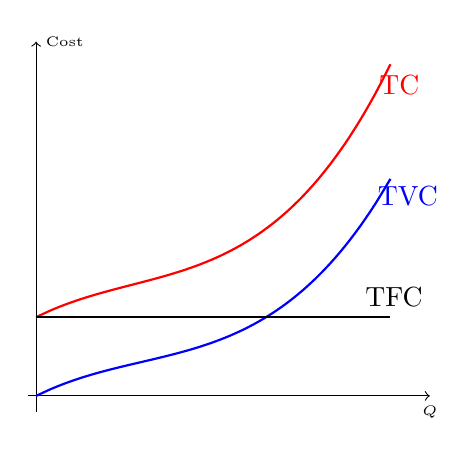
\begin{tikzpicture}
    \draw[->](-0.1,0)--(5,0)node[left,below,font=\tiny]{$Q$};
    \draw[->](0,-0.2)--(0,4.5)node[right,font=\tiny]{Cost};
    % \foreach \x in {0,0.5,1}{\draw(\x,0)--(\x,0.05)node[below,outer sep=2pt,font=\tiny]at(\x,0){\x};}
    % \foreach \y in {1}{\draw(0,\y)--(0.05,\y)node[left,outer sep=2pt,font=\tiny]at(0,\y){\y};}
    % \draw[color=red, thick,smooth,domain=0:1]plot(\x,1);
    % \draw[color=red, thick,smooth,domain=-1:-0.02]plot(\x,0);
    \draw[color=blue, thick,smooth, domain=0:4.5, mylabel=at 0.9 above right with {TVC}]plot(\x, {0.05*\x^3-0.2*\x^2+0.5*\x});
    \draw[color=red, thick,smooth, domain=0:4.5, mylabel=at 0.9 above right with {TC}]plot(\x, {0.055*\x^3-0.2*\x^2+0.5*\x+1});
    \draw[color=black, thick,smooth, domain=0:4.5, mylabel=at 0.9 above right with {TFC}]plot(\x, 1);
    % \draw[color=red,smooth]circle(0.02);
    \end{tikzpicture}
    \caption{Cost curve}
    \label{fig:TC}
\end{figure}
Also, we can consider average quantity, such as $\mathrm{AFC} = \frac{\mathrm{TFC}}{Q}, \mathrm{AVC} = \frac{\mathrm{TVC}}{Q}$, even, marginal cost, $\mathrm{MC} = \frac{\Delta \mathrm{TC}}{\Delta Q}$.
\begin{figure}
        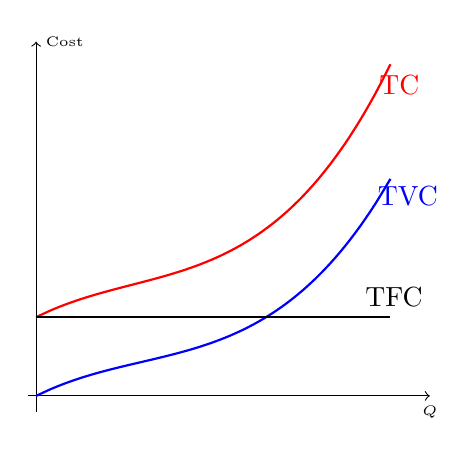
\begin{tikzpicture}
            \draw[->](-0.1,0)--(5,0)node[left,below,font=\tiny]{$Q$};
            \draw[->](0,-0.2)--(0,4.5)node[right,font=\tiny]{Cost};
            % \foreach \x in {0,0.5,1}{\draw(\x,0)--(\x,0.05)node[below,outer sep=2pt,font=\tiny]at(\x,0){\x};}
            % \foreach \y in {1}{\draw(0,\y)--(0.05,\y)node[left,outer sep=2pt,font=\tiny]at(0,\y){\y};}
            % \draw[color=red, thick,smooth,domain=0:1]plot(\x,1);
            % \draw[color=red, thick,smooth,domain=-1:-0.02]plot(\x,0);
            \draw[color=blue, thick,smooth, domain=0:4.5, mylabel=at 0.9 above right with {TVC}]plot(\x, {0.05*\x^3-0.2*\x^2+0.5*\x});
            \draw[color=red, thick,smooth, domain=0:4.5, mylabel=at 0.9 above right with {TC}]plot(\x, {0.055*\x^3-0.2*\x^2+0.5*\x+1});
            \draw[color=black, thick,smooth, domain=0:4.5, mylabel=at 0.9 above right with {TFC}]plot(\x, 1);
            % \draw[color=red,smooth]circle(0.02);
        \end{tikzpicture}
\end{figure}








\end{document}